\documentclass[%
master,    % тип документа
natbib,      % использовать пакет natbib для "сжатия" цитирований
subf,        % использовать пакет subcaption для вложенной нумерации рисунков
href,        % использовать пакет hyperref для создания гиперссылок
colorlinks,  % цветные гиперссылки
%fixint,     % включить прямые знаки интегралов
]{disser}

\usepackage[
a4paper, mag=1000,
left=2.5cm, right=1cm, top=2cm, bottom=2cm, headsep=0.7cm, footskip=1cm
]{geometry}

\usepackage[intlimits]{amsmath}
\usepackage{amssymb,amsfonts}

\usepackage[T2A]{fontenc}
\usepackage[utf8]{inputenc}
\usepackage[english,russian]{babel}
\ifpdf\usepackage{epstopdf}\fi
\usepackage[autostyle]{csquotes}
\usepackage{rotating}
% Шрифт Times в тексте как основной
%\usepackage{tempora}
\usepackage{setspace}
\usepackage{mathtools}
% альтернативный пакет из дистрибутива TeX Live
%\usepackage{cyrtimes}
\usepackage{listings}
% Шрифт Times в формулах как основной
%\usepackage[varg,cmbraces,cmintegrals]{newtxmath}
% альтернативный пакет
%\usepackage[subscriptcorrection,nofontinfo]{mtpro2}

% Плавающие рисунки "в оборку".
\usepackage{wrapfig}

% Номера страниц снизу и по центру
%\pagestyle{footcenter}
%\chapterpagestyle{footcenter}

% Точка с запятой в качестве разделителя между номерами цитирований
%\setcitestyle{semicolon}

% Использовать полужирное начертание для векторов
\let\vec=\mathbf
%______________________________-
\usepackage{lipsum}

%\usepackage{titlesec}
%\usepackage{spacing}
%\titleformat{\section}[block]{\color{blue}\Large\bfseries\filcenter}{}{1em}{}
% Номера страниц снизу и по центру
\pagestyle{footcenter}
\chapterpagestyle{footcenter}

% Точка с запятой в качестве разделителя между номерами цитирований
%\setcitestyle{semicolon}



% Переопределение стандартных заголовков
%\def\contentsname{Содержание}
%\def\conclusionname{Выводы}
%\def\bibname{Литература}

\usepackage{geometry} % пакет для установки полей
\geometry{top=1.5cm} % отступ сверху
\geometry{bottom=2cm} % отступ снизу
\geometry{left=3cm} % отступ справа
\geometry{right=1.5cm} % отступ слева
\newcommand{\sectionbreak}{\clearpage}
\newcommand*{\No}{\textnumero}
\renewcommand{\Re}{\mathrm{Re}}
\renewcommand{\Im}{\mathrm{Im}}

\newcommand{\const}{\mathrm{const}}
\newcommand{\arccosh}{\mathrm{arccosh}}

\newcommand{\vF}{\mathbf{F}}
\newcommand{\ve}{\mathbf{e}}
\newcommand{\vk}{\mathbf{k}}
\newcommand{\vq}{\mathbf{q}}
\newcommand{\vp}{\mathbf{p}}
\newcommand{\va}{\mathbf{a}}
\newcommand{\vP}{\mathbf{P}}
\newcommand{\vK}{\mathbf{K}}
\newcommand{\vQ}{\mathbf{Q}}
\newcommand{\vA}{\mathbf{A}}
\newcommand{\vr}{\mathbf{r}}
\newcommand{\vR}{\mathbf{R}}

\newcommand{\vRR}{\boldsymbol{\mathcal{R}}}
\newcommand{\veps}{\boldsymbol{\varepsilon}}

\newcommand{\cA}{\mathcal{A}}
\newcommand{\cR}{\mathcal{R}}
\newcommand{\cM}{\mathcal{M}}
\newcommand{\cE}{\mathcal{E}}
\newcommand{\cJ}{\mathcal{J}}
\newcommand{\cT}{\mathcal{T}}
\newcommand{\cD}{\mathcal{D}}


%______________________________-
% Включать подсекции в оглавление
\setcounter{tocdepth}{2}

\graphicspath{{fig/}}

\begin{document}
\title{Моделирование нуклеосинтеза в звездах}
\maketitle
\section*{\centering Введение}
\addcontentsline{toc}{section}{Введение}
Данная работа рассматривает процесс синтеза ядер, а именно возникновение элементов в ходе эволюции нейтронной звезды. Преобразования, приводящие к появлению легких элементов (легче железа) известны и хорошо изучены. Распространенность элементов, расположенных в области за железом, относительно слабо зависит от массового числа A. Это свидетельствует об изменении механизма образования этих элементов.  Образование их в результате взаимодействия заряженных частиц сильно подавлено из-за кулоновского барьера. Фактор, который также необходимо принять во внимание, состоит в том, что большинство тяжелых элементов являются $\beta$-радиоактивными. По современным представлениям тяжелые элементы образуются в реакциях захвата нейтронов. Обычно различают быстрый (r) и медленный (s) процессы захвата нейтронов (от английских слов rapid и slow). Эти два механизма различаются отношением скорости захвата нейтронов (реакция (n, $\gamma$)) к скорости бета-распада. По современным представлениям примерно половина наблюдаемого количества элементов с A > 60 образуется в результате s-процесса. В настоящее время общепризнанно, что многие ядра тяжелее железа, включая все ядра тяжелее $^{209}Bi$, образуются в r-процессе путем быстрого последовательного захвата большого количества нейтронов. Главное условие - скорость захвата нейтронов должна быть больше скорости $\beta$-распада. 

Однако есть также некоторые элементы, возникновение которых не может происходить через эти процессы. Такие элементы являются обойденными. 

В данной работе, будут моделироваться реакции, приводящие к появлению обойденных ядер, а именно - столкновительный $\beta$-распад, с использование открытой библиотеки реакций REACLIB, в основе которой лежит построение сечения зависимостью от температуры по 7 параметрам. Данная библиотека уже включает в себя некоторый набор реакций, приводящий к появлению обойденных ядер, но в данной работе нас интересует исследование только влияние СБР на эволюцию системы. 

Основной целью работы является построение сечений для столкновительного $\beta$-распада для столкновении элементов с протоном, а также оценка влияния этих реакций на полученную распространенность элементов в результате всех процессов за промежуток времени.

Сам процесс моделирования будет выполняться с помощью открытой библиотеки SkyNet, написанную Jonas Lippuner с дополнение ее своим набором реакций.

\section{Нуклеосинтез Большого Взрыва}

\begin{figure}[h]
	\center{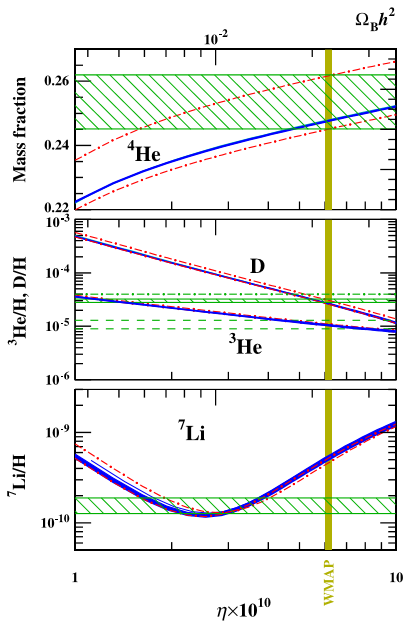
\includegraphics[width=0.7\linewidth]{2}}
	\caption{Вычисленная распространенность 4He, D, 3He и 7Li (синие линии) в зависимости от отношения барион-фотон $\eta$. Зеленые области - наблюдаемые концентрации, а желтая вертикальная полоса - наблюдаемое значение $\eta$. Вычисленные количества 4He, D и 3He согласуются с наблюдениями, но прогнозируется избыток 7Li в 4-5 $\sigma$. Это известная «литиевая проблема». Рисунок 1 из Cocetal. (2013)}
	\label{ris:Cocetal}
\end{figure}

Нуклеосинтез большого взрыва (BBN) произвел в основном водород (~ 75$\%$ общей массы) и гелий (~ 25$\%$) в период от первых десяти секунд до минуты после Большого взрыва, а также некоторое количество дейтерия, 3He и 7Li \cite{Tytler}. 13,8 Gyr позже химический состав Вселенной оставался около 75$\%$ H и 25$\%$ He, потому что создание более тяжелых элементов требует экстремальных физических условий. Интересно, что BBN является проблемой для моделирования, потому что он включает лишь небольшое количество ядер. В настоящее время существуют большие расхождения между результатами моделирование BBN и наблюдениями. Прогнозируемый дейтерий и распространенность 4He хорошо согласуется с наблюдениями, но модели BBN предсказывают большую распространенность 7Li на 4-5 $\sigma$ по сравнению с наблюдениями, см. рис. \ref{ris:Cocetal}, которая изображена на рисунке 1 от Coc et al. (2013). Это расхождение не до конца изучено и называется «литиевой проблемой». Предлагаемые причины включают систематические ошибки в наблюдениях численности 7Li, неизвестные или плохо измеренные ядерные свойства $^{7}Be$ и даже неизвестные физические процессы, протекающий за гранью Стандартной модели.

\section{Столкновительный $\beta$-распад}
Данный процесс является одним из процессов, приводящих к появлению обойденных ядер.

Обойдённые ядра - устойчивые атомные ядра, лежащие в стороне от всех возможных путей образования тяжёлых ядер из более лёгких в процессе последовательного захвата последними нейтронов \cite{reactions}. Распространённость обойденных ядер, как правило, примерно на два порядка величины ниже, чем у близких к ним ядер, лежащих на пути нейтронного захвата. К таковым относятся: $^{74}Se$, $^{78}Kr$, $^{80}Kr$, $^{84}Sr$, $^{92}Mo$, $^{94}Мо$, $^{96}Ru$, $^{98}Ru$, $^{102}Pd$, $^{106}Cd$, $^{108}Cd$, $^{113}In$, $^{112}Sn$, $^{114}Sn$, $^{115}Sn$, $^{120}Te$, $^{124}Xe$, $^{126}Xe$, $^{130}Ba$, $^{132}Ba$, $^{136}Ce$, $^{138}Ce$, $^{144}Sm$, $^{152}Gd$, $^{152}Dy$, $^{158}Dy$, $^{162}Er$, $^{164}Er$, $^{168}Yb$, $^{174}Hf$, $^{180}W$, $^{184}Os$, $^{190}Pt$, $^{196}Hg$ \cite{role}.

Столкновительный $\beta-$распад стабильных ядер, инициируемый их кулоновскими столкновениями с другими ядерными частицами звездной среды, может быть основой модели процесса синтеза обойденных ядер.
Проблема их синтеза на основе физического механизма захвата нейтронов ($s-$ или $r-$процесса) состоит в прерывании цепочки последовательных $\beta-$распадов на $\beta$-стабильном ядре $(A,Z)$.

Процесс СБР стабильных ядер, о котором говорилось выше, для нуклидов главной последовательности предоставляет еще одну возможность преодолеть энергетический порог и осуществить переход 
$$(A,Z) \xrightarrow[]{\beta^-} (A,Z + 1)$$
, открывая путь к последующему естественному $\beta$-переходу
$$(A,Z+1) \xrightarrow[]{\beta^-} (A,Z + 2)$$

Может оказаться, что при этом малость сечений для процесса такого рода уже не будет играть особой роли, если будут не малы плотность вещества в недрах звезды и временная протяженность квазиравновесной стадии звездной эволюции.

Расчеты показывают, что модель синтеза обойденных элементов в звездном веществе на этапе квазиравновесной стадии, основанная на явлении СБР стабильных ядер главной последовательности, качественно, а в ряде случаев и количественно, способна воспроизвести нерегулярный ход кривой относительной распространенности обойденных ядер. Этот факт можно расценивать как косвенное свидетельство в пользу реальности явления столкновительного $\beta$-распада стабильных ядер \cite{tak}.

В случае столкновительного $\beta$-распада возможно несколько видов процессов, а именно: протон-ядерные, ядро-ядерные и процесс, стимулированный нейтронами. Рассчитанные сечения для протон-ядерных и ядро-ядерных оказались невелики (менее $10^{-50}cm^2$), и процесс пока не доступен для прямого наблюдения, но при помощи программного обеспечения, позволяющего моделировать данные процессы мы можем оценить влияние их на конечные распространенности элементов \cite{tak_article}. Наряду с кулоновскими столкновениями ядер можно предложить механизм СБР, не связанный с кулоновскими силами и в то же время незамаскированный возможным появлением продуктов $\beta$-распада за счет ядерных реакций. Речь идет о процессе СБР ядра, стимулированном столкновениями с нейтронами.

Данная работа рассматривает в первую очередь влияние протон-ядерного столкновения на процессы, протекающие в нейтронных звездах, а именно r-process, так как концентрация протонов при этом достаточно велика, чтобы это влияние оказалось существенным. 

Сечение для столкновительного $\beta$ распада получим через формулу (\ref{eq:sbr}).

\begin{equation}
\label{eq:sbr}
\begin{split}
P_{\beta}\left((A, Z) \to (A, Z + 1)\right) = \left(\frac{8}{\pi\mu_{A A'} T^3}\right)^{1/2} \times \\
\times \int_{\Delta + \Delta_f + 1}\sigma_\beta^{(col)}(\beta_f)\exp(-\epsilon/T)\epsilon d \epsilon
\end{split}
\end{equation}

В данной формуле $\sigma_\beta^{(col)}$ представляет из себя (\ref{eq:sigma}): 

\begin{equation}
\label{eq:sigma}
\begin{split}
\sigma_\beta^{(col)}(\beta_f) =
\frac{4\sqrt{2}}{\pi}\frac{g_v^2\alpha_e^4 Z (Z + 1)Z'^4\mu^{9/2}}{\epsilon_i^{3/2}(1-\exp(-2\pi\lambda_i))}\xi_\beta(\beta_f) \times \\
\int_{0}^{\xi_i-\Delta-\Delta_f}\frac{\Phi(E_f)d\epsilon_f}{(\exp(2\pi\lambda_f)-1)k_f(k_i-k_f)^4(k_i+k_f)^2} \times \\
\int_{x_0}^{0}\frac{\left|F(-i\lambda_i,-i\lambda_f,1;x)\right|^2}{(1-x)^2}dx,
\end{split}
\end{equation}

где $E_f = \epsilon_i - \epsilon_f - \Delta - \Delta_f$, $x_0 = -4 k_i k_f / (k_i - k_f)^2$, а функция $\Phi(E)$ имеет вид (\ref{eq:phi}):

\begin{equation}
\label{eq:phi}
\Phi(E) = \frac{1}{60}(E^2-1)^{1/2}(2E^4-9E^2-8)+\frac{1}{4}E\ln(E+(E^2-1)^{1/2})
\end{equation}

\begin{equation}
\label{eq:lambda}
	\lambda_i = \frac{ZZ'e^2\mu}{\hbar^2 k_i}, \lambda_f = \frac{(Z+1)Z'e^2\mu}{\hbar^2 k_f}
\end{equation}

\begin{equation}
\label{eq:epsilon}
\epsilon_i = \frac{\hbar^2 k_i^2}{2\mu}, \epsilon_f = \frac{\hbar^2 k_f^2}{2\mu}
\end{equation}

Для возможности использования полученных сечений вместе с другими библиотеками ядерных реакций необходимо привести их к единому формату. Данным форматом был выбран REACLIB.

\section{REACLIB}

База данных JINA REACLIB представляет из себя список ядерных реакций. Для каждой реакции в библиотеке представлен ее тип (chapter), выражающий количество участников, который может быть:
\begin{itemize}
	\item 1 участник, 1 продукт
	\item 1 участник, 2 продукта
	\item 1 участник, 3 продукта
	\item 2 участника, 1 продукт
	\item 2 участника, 2 продукта
	\item 2 участника, 3 продукта
	\item 2 участника, 4 продукта
	\item 3 участника, 1 продукт
	\item 3 участника, 2 продукта
	\item 4 участника, 2 продукта
	\item 1 участника, 4 продукта
\end{itemize}
 База полностью открыта и доступна для сообщества через интернет. Текущая версия библиотеки хранит показатели реакций, таких как зависимость от температуры через семи-параметрическое приближение \cite{jina}, тип реакции (резонирующая, нерезонирующая, слабая, спонтанный распад), значение температуры, переданное среде, а также параметр "v", указывающий, являются ли показатели $a_0, .., a_6$ обратными. В подавляющем большинстве реакций показатели представляют из себя параметризацию сечения в зависимости от температуры:

$$\lambda = \exp \bigg[a_0 + \sum_{i=1}^{5}a_iT_9^{\frac{2i-5}{3}}+a_6 \ln T_9\bigg]$$

Чтобы получить параметры $a_0, .., a_6$ для каждой из наших реакций мы воспользуемся статистической моделью.

Модель представляет из себя усредненные коэффициенты перехода T. Они не отражают резонансное поведение, но описывают эффект поглощения чере мнимую часть в (оптическом) ядро-ядро потенциале, что приводит к известному выражению:


\begin{multline}
\sigma^{\mu\nu} = \\
= \frac{\pi\hbar/(2\mu_{ij}E_{ij})}{(2J_i^\mu+1)(2J_j+1)}\sum_{J,\pi}(2J + 1) \\
\times \frac{T_j^\mu(E,J,\pi,E_i^mu, J_i^\mu,\pi_i^\mu)T_0^\nu(E,J,\pi,E_m^\mu,J_m^\nu,\pi_m^\nu)}{T_{tot}(E,J,\pi)}
\end{multline}

для сечения $\sigma^{\mu\nu}$ реакции $i^\mu(j,o)m^\mu$ из состояния $i^\mu$ в состояние $m^\nu$ конечного ядра с центром энергии масс $E_{ij}$ и уменьшенной массой $\mu_ij$.

Показатели реакций были посчитаны для набора из 24 температур: $T_9$ = 0.1,0.15, 0.2, 0.3, 0.4, 0.5, 0.6, 0.7, 0.8, 0.9, 1.0, 1.5, 2.0, 2.5, 3.0, 3.5, 4.0, 4.5, 5.0, 6.0, 7.0, 8.0, 9.0, 10.0 ($T = T_9 \times 10^{9}\text{К}$))Для простого применения в астрофизических исследованиях все виды реакций ($(n,\gamma)$, $(n,p)$, $(p,\alpha)$, $(p, \gamma)$, (p, n), $(p, \alpha)$, $(\alpha, \gamma)$, $(\alpha, n)$, $(\alpha, p)$, $(\gamma, n)$, $(\gamma, p)$, $(\gamma, \alpha))$ аппроксимируются через единое приближение вида

\begin{equation}
\label{eq:system}
\begin{split}
\left.
	\begin{array}{ccc}
		N_{A}\langle \sigma v \rangle \\
		\lambda_\gamma
	\end{array}
\right\}
 = \exp (a_0 + a_1 T_9^{-1} + a_2 T_9^{-1/3} + \\
a_3 T_9^{1/3} + a_4 T_9 + a_5 T_9^{5/3} + a_6 \ln T_9)
\end{split}
\end{equation}

c 7 открытыми параметрами $a_0$ - $a_6$, где $T_9$ это $10^9$К.

Данное приближение является достаточно гибким чтобы удовлетворить различным температурным зависимостям для различных видов реакций в промежутке температур $0.001 \le T_9 \le 10$ \cite{rates}.

\section{SkyNet}

Программный пакет SkyNet представляет из себя обще-целевую сеть ядерных реакций, специально разработанную для моделирования r-процесса, но она также применима к другим астрофизическим сценариям \cite{skynet}.

SkyNet написан на языке C++ и имеет модульную архитектуру. Помимо сети ядерных реакций, он также включает в себя модуль решения ядерного статистического равновесия (!!! Nuclear Statistical equilibrium), уравнение состояния Гельмгольца. SkyNet также моделирует эволюцию температуры, отслеживая изменение энтропии при ядерных реакциях и распадах.

SkyNet также имеет обертку для использования ее с Python, что делает очень удобным использование его через интерактивные оболочки.

Важно отметить, что SkyNet успешно прошел сравнения с другими аналогичным ПО (WinNet, XNet) и даже, приблизился к симуляции Seitenzahl \cite{simulation}.

При использовании данного пакета были внесены изменения в исходный код, а именно добавлена функцию для чтения файлов REACLIB нового формата не построчно, а набором из 4 строк, аналогичная которой была добавлена в исходный код самого проекта.

(!!! мало информации, нужно найти больше)

\section{Построение СБР}

Итак, мы пришли к тому, что для добавления новых реакций СБР мы должны построить сечение по формуле (\ref{eq:sbr}). Для упрощения расчетов, а именно, уменьшения количества операций, связанных с умножениями на константы, было принято решение перейти к системе единиц СГС ($m_e = \hbar = c = 1$). Тогда $\alpha = \frac{e}{\hbar_c}$. Таким образом, (\ref{eq:lambda}) принимает вид

\begin{equation}
\lambda_i = \frac{Z Z' e^2 \mu}{\hbar^2 k_i} = \frac{Z Z' e^2 \mu}{\sqrt{2\mu \epsilon_i}} = Z Z' e^2 \sqrt{\frac{\mu}{2 \epsilon_i}} = Z Z' \alpha \sqrt{\frac{\mu}{2 \epsilon_i}}
\end{equation}

\begin{equation}
\lambda_f = \frac{(Z+1) Z'  e^2 \mu}{\hbar^2 k_f} = (Z + 1)Z' e^2 \sqrt{\frac{\mu}{2 \epsilon_f}} = Z Z' e^2 \sqrt{\frac{\mu}{2 \epsilon_i}} = Z Z' \alpha \sqrt{\frac{\mu}{2 \epsilon_i}}
\end{equation}

\begin{equation}
\mu = m_n \frac{A_1 A_2}{A_1 + A_2}
\end{equation}
, где $m_n$ =  $m_n/m_e = 1,835\times10^3 =$, $g_v = 2.9899 \times 10^{-12}$.

Для построение сечения, в таком случае, получаем множитель:

$$
	<\sigma \cdot v> \times 1.4915 \times 10^{-21} \cdot 2.998 \times 10^{10} = 	<\sigma \cdot v> \times 44,722 10^{-12}.
$$

Заметим также, что в формуле (\ref{eq:sigma}) присутствует гипергеометрическая функция вида $F(-i\lambda_i,-i\lambda_f,1;x)$. Для ее вычисления будем использовать библиотечную функцию из пакета \textbf{mpmath}. Вычисление этой функции сама по себе операция очень затратная по производительности, но также на различных значениях параметров могут получаться недостаточно точные значения. Это зависит от того, какой алгоритм был использован. Поэтому в начальной версии программы, получающей сечение СБР была заложена проверка корректности вычисления. 

С учетом известного преобразования гипергеометрической функции (\ref{eq:hyp-check}), при каждом вычислении ее было также получено значение этой функции для параметров в правой части выражения. Затем полученные значения сравнивались друг с другом и модуль их абсолютной разницы не должен был превышать $10^{-11}$. 

В текущей версии программы данная проверка была отключена, чтобы ускорить процесс вычислений, но мы убедились что на интересующем нас промежутке значение функции через библиотечную реализацию получено верно (для заданной точности).

\begin{equation}
\label{eq:hyp-check}
F(a,b,c;x) = (1-x)^{-a}F\left(a,c-b,c; \frac{x}{x-1}\right)
\end{equation}

Формула (\ref{eq:sigma}) также включает в себя матричный элемент $\xi_b(\beta_f)$, который является безразмерной величиной. Данный параметр, как и прочие, необходимые для работы программы, были получены ранее \cite{tak}. Причем в указанной работе вместо матричного элемента представлен параметр $\lg f_0 t$, из которого можно перейти к  $\xi_b(\beta_f)$.

$$
\lg f_0 t \equiv \beta, f_0 t = 10^\beta
$$

$$
\xi_b(\beta_f) = \frac{6250}{10^\beta}
$$

Программа для построения сечения СБР с протоном работает с наборами входных параметров, таких как \textbf{[78.0, 34.0, 3.5737, 0.0, 4.8, 'se', 'br']}. Данный набор представляет из себя переход (\ref{eq:transform-1}).

\begin{equation}
\label{eq:transform-1}
^{78}Se \xrightarrow[\lg f_0 t = 4.8]{\Delta = 0.879 MEv}  \ ^{78}Br
\end{equation}

Для всех реакций, для которых в данной работе было построено сечение, присутствует также параметр $\Delta_f$, равный нулю, потому что присутствие его в переходе значительно снижает вероятность этого перехода и, для оценки влияния СБР на общую картину эволюции, переходами такого рода можно пренебречь.

В связи с переходом в другую систему единиц, помимо множителя для (\ref{eq:sbr}),  мы также должны преобразовать входные параметры для перехода в иную систему координат ($\text{МэВ} = 0.511 $!!!), а именно

$$
t^{\text{СГС}} = t^{\text{СИ}} * \frac{1.16}{\text{МэВ}} \times 10^{-10},
$$
$$
\Delta^{\text{СГС}} = \frac{\Delta^{\text{СИ}}}{\text{МэВ}}, \Delta_f^{\text{СГС}} = \frac{\Delta_f^{\text{СИ}}}{\text{МэВ}}.
$$

Последние 2 параметра ('se', 'br') представляют собой вручную заданные названия элементов, первый - праматеринское ядро, второй - материнское. Используются для записи построенных сечений в файл. 

Рассмотрим, например, сечение для перехода 
$$^{130}Xe \to ^{130}Cs.$$

В результате работы программы, получаем график сечения  (рис. \ref{ris:1}).

\begin{figure}
	\center{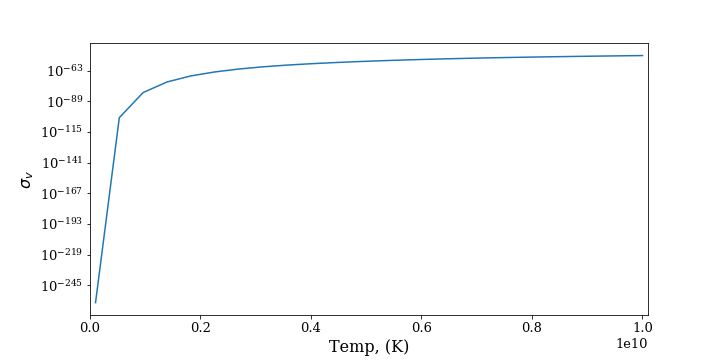
\includegraphics[width=0.8\linewidth]{xe130-cs130}}
	\caption{Сечение для СБР при столкновении $^{130}Xe$ с протоном}
	\label{ris:1}
\end{figure}

Важно отметить, что при вычислении СБР в начале искомого отрезка температуры ($\text{~}10^8\text{с}$), возникали ситуации деления на очень малый аргумент. Из-за этого на граничной слева температуре построенное сечение нельзя назвать точным из-за погрешностей округления, но поскольку, как мы знаем, SkyNet игнорирует реакции с небольшим сечением для даной температуры, данные погрешности не имеют смысла из-за пренебрежимо малого сечения ($\ll 10^{-100} \frac{\text{см}^2}{\text{с}}$).

\section{Анализ результатов}
В данной работе мы построили сечение СБР для столкновения всех элементов из списка (!!!) с протоном (рис. \ref{ris:sigma-full}, \ref{ris:sigma-full-2}).

\begin{sidewaysfigure}
 	\center{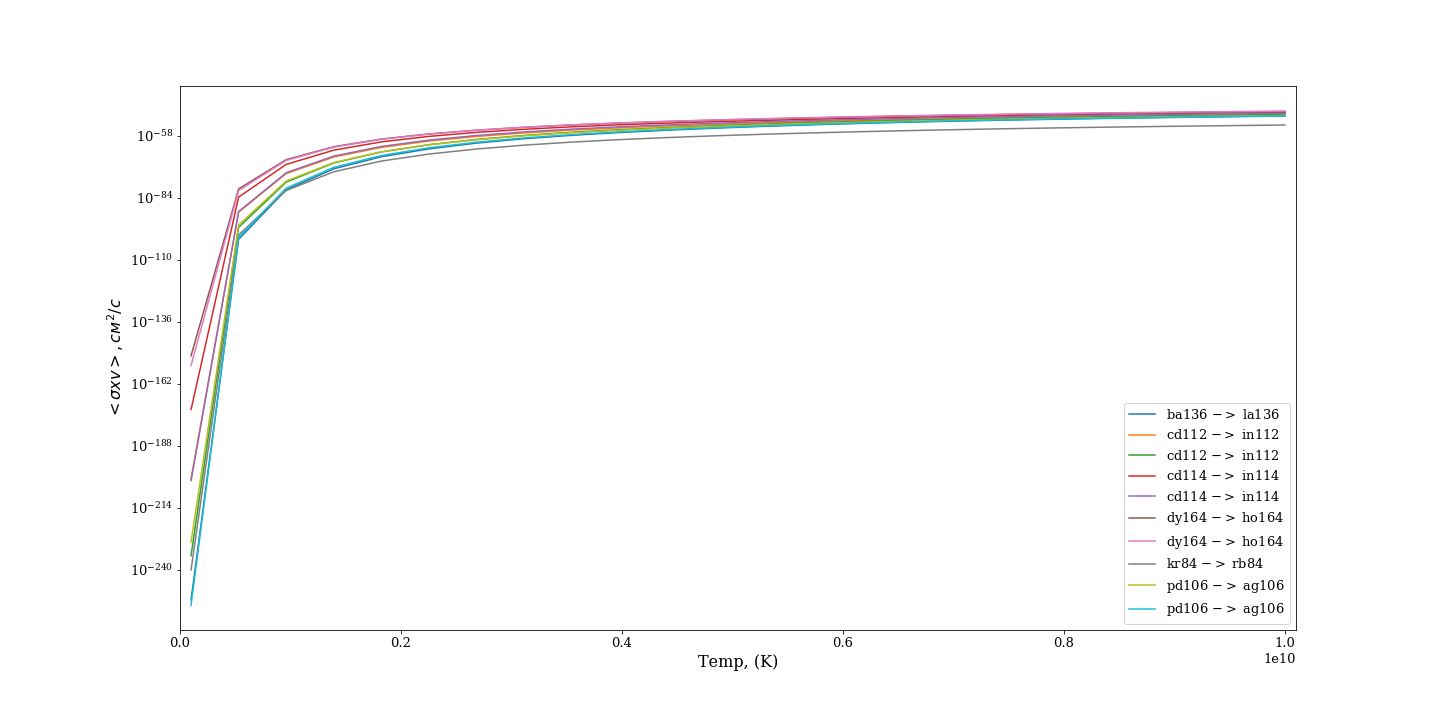
\includegraphics[width=1\linewidth]{sigma-full}}
 	\caption{Сечение для СБР при столкновении ядер ($^{136}Ba, ^{112}Cd, ^{114}Cd, ^{164}Dy, ^{84}Kr, ^{106}Pd$) с протоном}
 	\label{ris:sigma-full}
\end{sidewaysfigure}
\begin{sidewaysfigure}
	\center{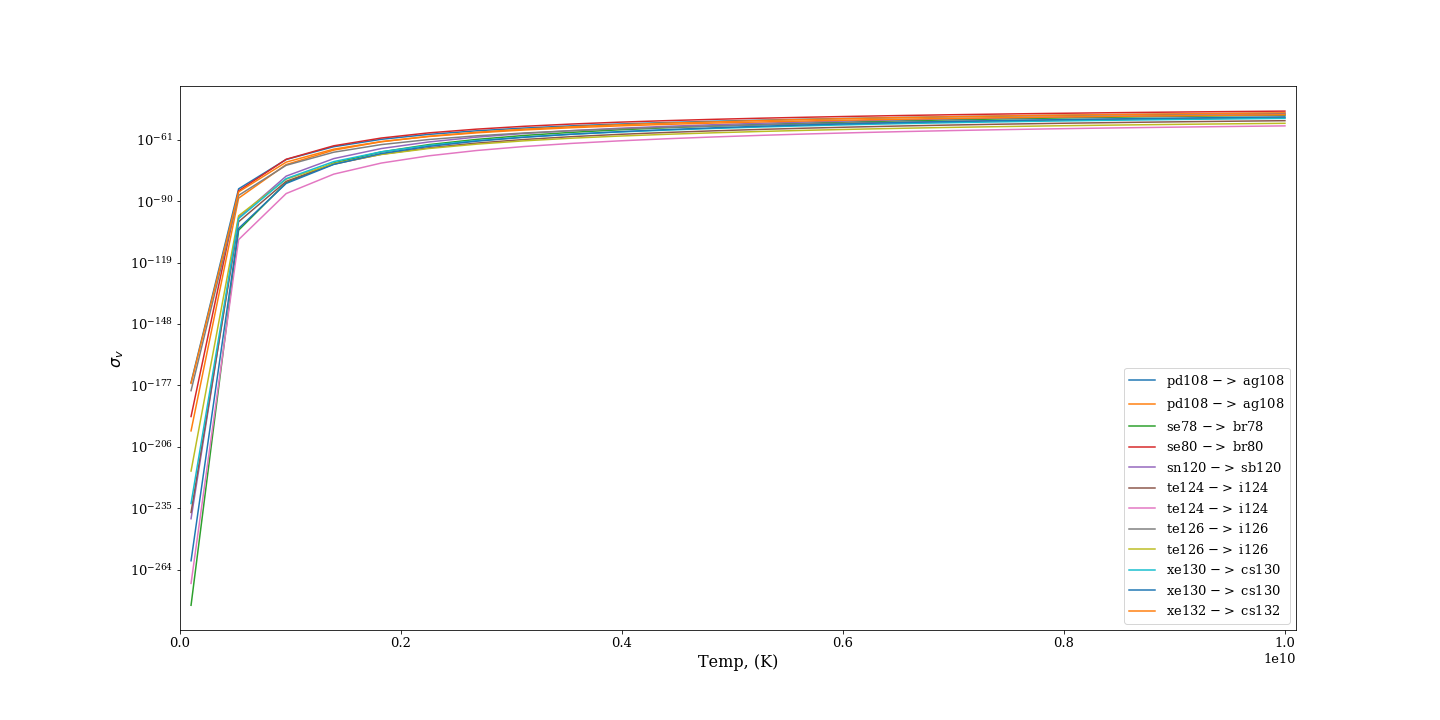
\includegraphics[width=1\linewidth]{sigma-full-2}}
	\caption{Сечение для СБР при столкновении ядер ($^{108}Pd, ^{78}Se, ^{80}Se, ^{120}Sn, ^{124}Te, ^{126}Te, ^{130}Xe, ^{132}Xe$) с протоном}
	\label{ris:sigma-full-2}
\end{sidewaysfigure}

Полученные 24 значения температур являются избыточными в нашем случае, так целью является параметризация данной зависимости через 7 параметров $a_0, ..., a_6$ (\ref{eq:system}). То есть мы имеет 17 лишних уравнений. Поэтому для решения переопределенной системы воспользуемся методом наименьших квадратов (\ref{ris:2}).

\begin{figure}[h]
	\center{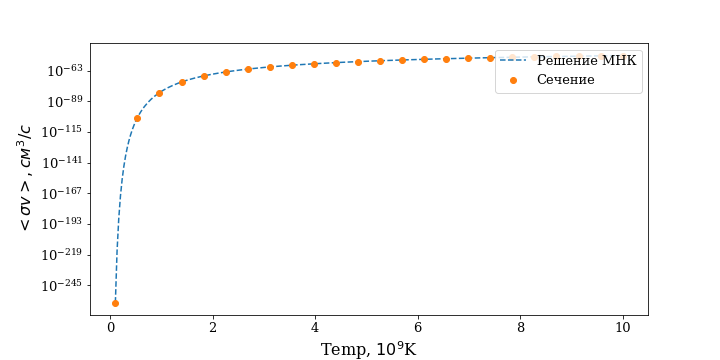
\includegraphics[width=0.8\linewidth]{compare-xe130-cs130}}
	\caption{Сравнение решения методов наименьших квадратов с полученным сечением}
	\label{ris:2}
\end{figure}

Далее, составим необходимый для REACLIB файл библиотеки реакций. Для перехода $^{130}Xe \to ^{130}Cs$ получаем строки вида: 

\begin{lstlisting}[label={lst:label}]
	5
	         pxe130cs130    p                  cleaw     0.00000e+00          
	 3.631089e+01-2.513083e+01-3.379005e+02 1.434772e+02                      
	-2.028014e+00-6.306473e-02-1.208779e+02                                   
	
\end{lstlisting}

В данном файле стоит отметить факт явного указания $p$ - протона в качестве участника реакции, так как сечение СБР зависит от концентрации протонов. 

Построим также графическое представление параметров $a$ для всех перечисленных выше (!!!) реакций  (рис. \ref{ris:a-1} - \ref{ris:a-4}).

\begin{sidewaysfigure}
	\center{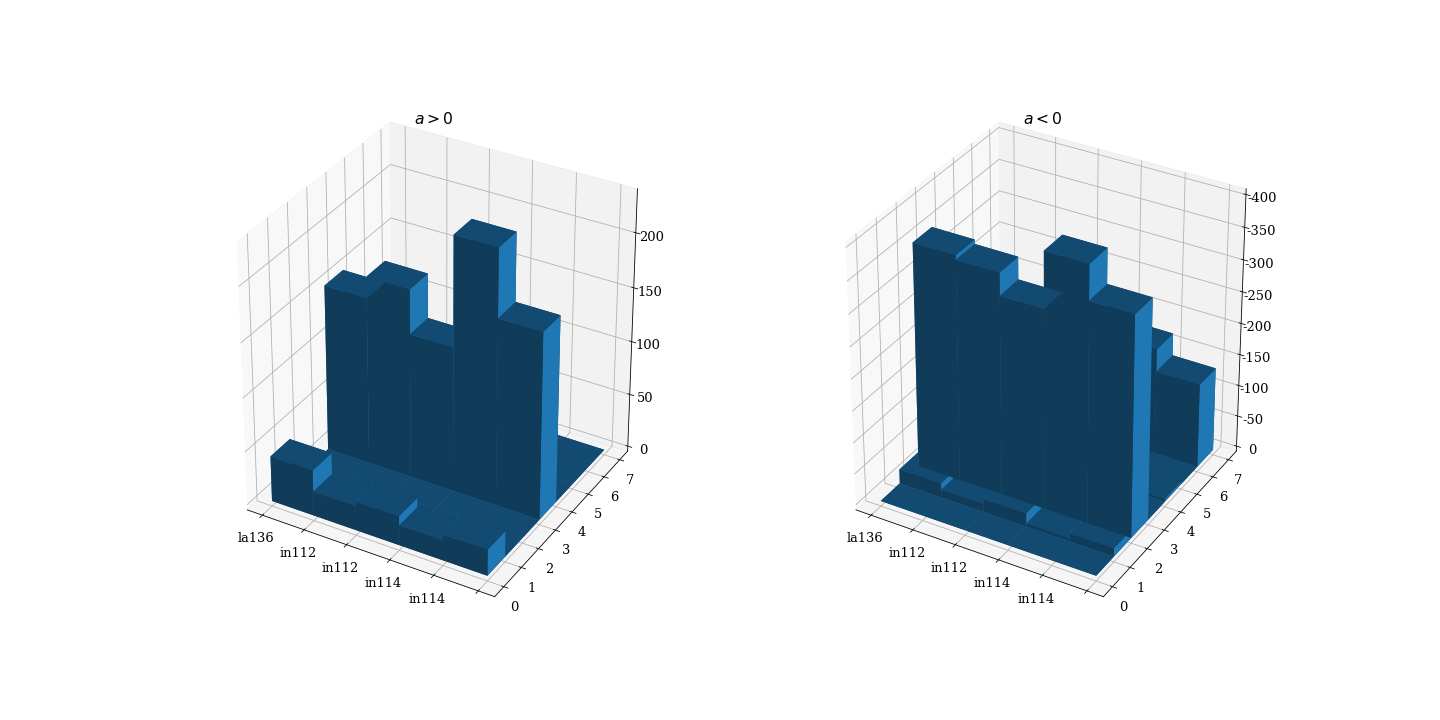
\includegraphics[width=1\linewidth]{a-1}}
	\caption{Значения параметров $a$ для столкновения протона с $^{136}Ba, ^{112}Cd, ^{114}Cd$}
	\label{ris:a-1}
\end{sidewaysfigure}
\begin{sidewaysfigure}
	\center{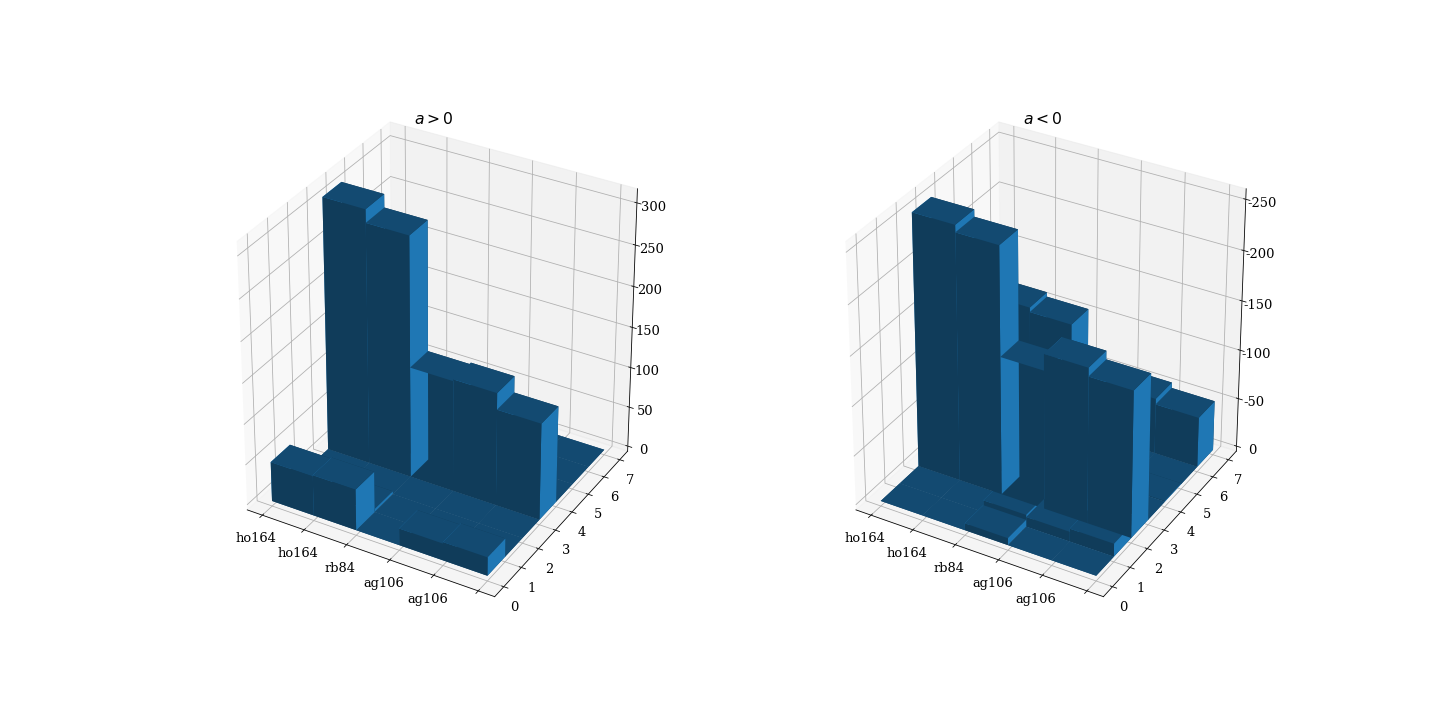
\includegraphics[width=1\linewidth]{a-2}}
	\caption{Значения параметров $a$ для столкновения протона с $^{164}Dy, ^{84}Kr, ^{106}Pd$}
	\label{ris:a-2}
\end{sidewaysfigure}
\begin{sidewaysfigure}
	\center{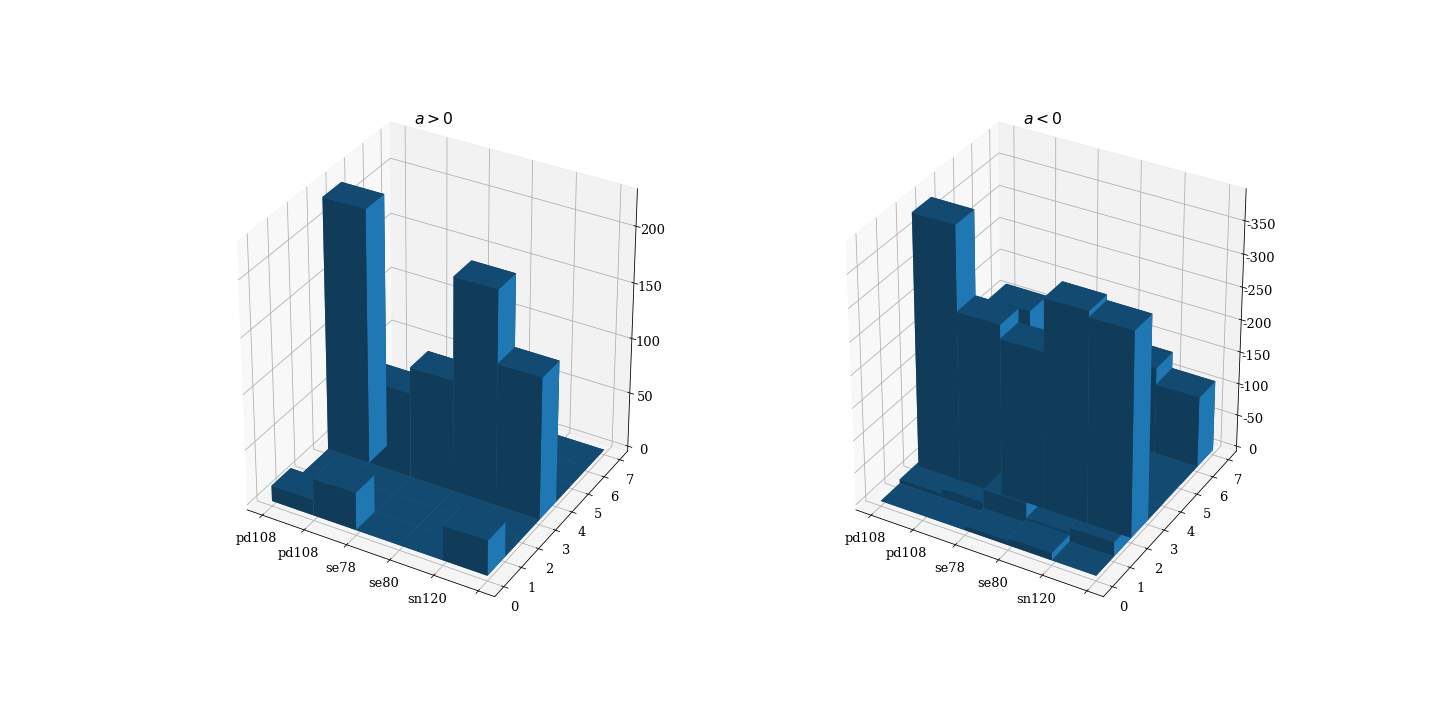
\includegraphics[width=1\linewidth]{a-3}}
	\caption{Значения параметров $a$ для столкновения протона с $^{108}Pd, ^{78}Se, ^{80}Se, ^{120}Sn$}
	\label{ris:a-3}
\end{sidewaysfigure}
\begin{sidewaysfigure}
	\center{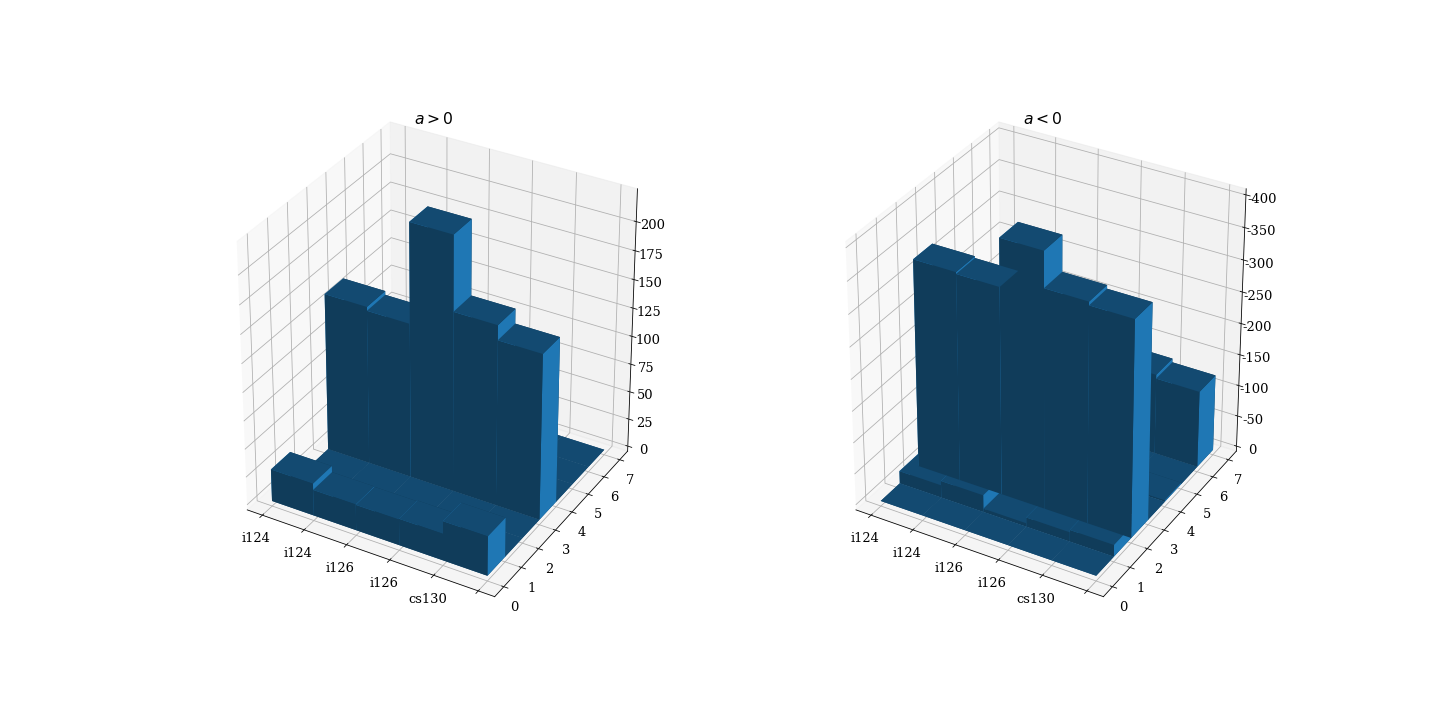
\includegraphics[width=1\linewidth]{a-4}}
	\caption{Значения параметров $a$ для столкновения протона с $^{124}Te, ^{126}Te, ^{130}Xe$}
	\label{ris:a-4}
\end{sidewaysfigure}

Для моделирования ядерных реакций воспользуемся включенной в SkyNet моделю r-process. Она содержит список из 7836 ядер, участвующих в реакциях, начальные распространенности этих ядер, а также зависимости плотности и температуры от времени. Эволюция протекает в промежутке времени от $1.21\times 10^{-3}c$ до $5\times 10^8c$. 

Изначально, если оставлять файл JINA REACLIB в таком виде, в котором он присутствует в библиотеке, влияние добавленных мною реакций отсутствовало. Это связано с тем, что в сети уже присутствовали реакции с этими элементами, но гораздо большим сечением, которое перекрывает наши реакции. Добится хоть какого-то влияния на небольших температурах невозможно, так как по характеру графика на рисунке (\ref{ris:1}) можно заметить его быстрое затухание при стремлении температуры справа к $10^8 K$, а именно при относительно низких ($10^9 K$) температурах протекает большая часть эволюции.

Для того, что проверить влияние, было решено учесть только те реакции, приводящие к образованию обойденных ядер, которые представляют из себя разрешенный $\beta$-распад. Для этого из библиотеки REACLIB были исключены реакции вида (\ref{eq:remove1}), то есть 168 реакций.

\begin{equation}
\label{eq:remove1}
	^{79}Br \to ^{78}Br + n
\end{equation}

Полученные данные представляют из себя иерархический формат данных h5. Извлекая конечные распространенности, видим результат для всех обойденных ядер (рис. \ref{ris:result}):

\begin{sidewaysfigure}[h]
	\center{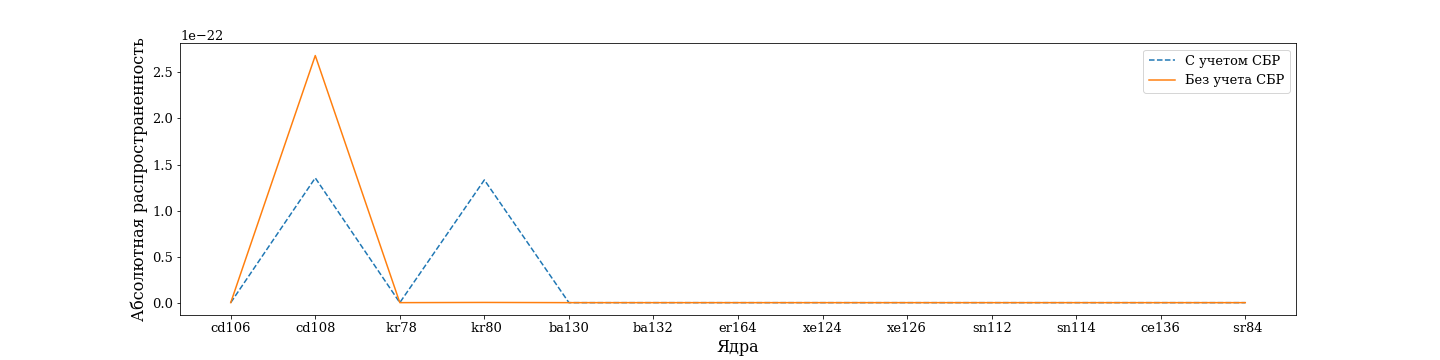
\includegraphics[width=1\linewidth]{result}}
	\caption{Конечные распространенности обойденных ядер}
	\label{ris:result}
\end{sidewaysfigure}

Построим график относительной ошибки между эволюцией элементов с нашей библиотекой реакций и тем, что присутствовало в изначальной версии REACLIB (рис. \ref{ris:result-err}):

\begin{sidewaysfigure}[h]
	\center{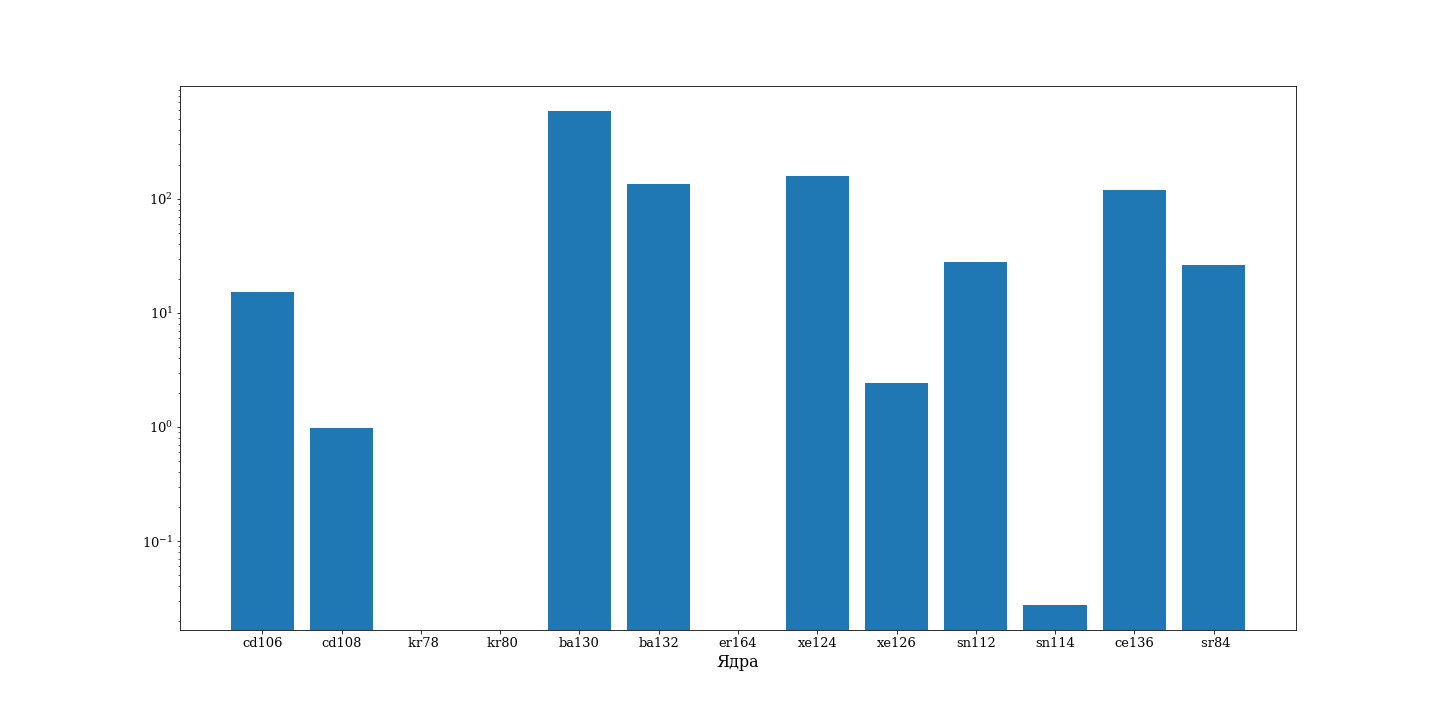
\includegraphics[width=1\linewidth]{result-err}}
	\caption{Относительная ошибка при сравнении стандартной библиотеки реакций SkyNet и библиотеки, учитывающей только СБР для образования обойденных изотопов}
	\label{ris:result-err}
\end{sidewaysfigure}

С учетом того, что мы полностью удалили все реакции, приводящие к возникновению обойденных $\beta$ ядер из сети реакций, полученная разница в их распространенностях оказалась не так велика, что говорит о том, что наши реакции действительно учитывались и смогли смоделировать возникновение некоторого количества обойденных ядер.

\section{Заключение}

В данной работе было рассмотрено влияние столкновительного бета распада на эволюцию звездных процессов. На языке Python был получено сечения для столкновительного процесса некоторых ядер с протоном. При помощи программного пакета SkyNet, а также дополнения библиотеки JINA REACLIB было подтверждено, что СБР может являться источником обойденных ядер и при больших значениях сечения это влияние существенно, но конкретно для ситуации столкновения с протоном, это влияние невелико даже для r-процесса. Чтобы увидеть эти изменения, пришлось учесть только реакции, приводящие к образованию обойденных ядер, которые представляют из себя разрешенный $\beta$-распад

Данная работа рассматривает только часть образований материнских ядер, причем при столкновении с протоном. Также, для расширения списка реакций необходимо добавить столкновительные реакции для других ядер, а также нейтронов, сечения для которых намного выше, ввиду отсутствия Кулоновского барьера.

\bibliographystyle{utf8gost705u}
\bibliography{sample}
\end{document} 